\chapter{Design Realization} \label{ch:designRealization}
Evaluating the concept design from \autoref{ch:overview} it is seen that the concept has four bands-pass filters and one high-pass that needs to be designed. 
\begin{figure}[H]
\centering
\tikzsetnextfilename{SystemOverview}
\scalebox{0.8}{
\begin{circuitikz}
%% TOP BAND %% 
\node[] (AudioIN) at (-0.5,0) {Audio in};
\node[] (AudioIN) at (0,0) {};
\node[summation] (Summation) at (12.5,0) {};
\node[summation] (Summation2) at (12.5,-2) {};
\node[summation] (Summation3) at (12.5,-4) {};
\node[summation] (Summation4) at (12.5,-6) {};
\node[] (AudioOUT) at (14.5,0) {Audio out};
\draw[-] ($(AudioIN)+(1,0)$) -- ($(AudioIN)+(1,-8)$);
\draw[-] ($(AudioIN)+(1,0)$) -- ($(AudioIN)+(0.5,0)$);

%% Summation %%
\draw [->] (Summation2) -- node[at end,yshift=2mm,xshift=0mm]{\scalebox{0.5}{+}} (Summation);
\draw [->] (Summation) -- (AudioOUT);
\draw [->] (Summation3) -- node[at end,yshift=2mm,xshift=0mm]{\scalebox{0.5}{+}} (Summation2);
\draw [->] (Summation4) -- node[at end,yshift=2mm,xshift=0mm]{\scalebox{0.5}{+}} (Summation3);


%%% GUI %%
\node[gain] (GUI) at ($(7,1)+(AudioIN)$) {GUI};
\draw[->,red] ($(GUI)+(0.5,0.25)$) -- ($(GUI)+(1,0.25)$);
\draw[<-,blue] ($(GUI)+(0.5,-0.25)$) -- ($(GUI)+(1,-0.25)$);

\draw [->,red] ($(4,.25)+(AudioIN)$) -- ($(4.5,.25)+(AudioIN)$); %% add (.5,.25) to the coordinate

%% Second Band
\draw [->,red] ($(4,-1.75)+(AudioIN)$) -- ($(4.5,-1.75)+(AudioIN)$);
\draw [<-,blue] ($(7.7,-2.75)+(AudioIN)$) -- ($(8.2,-2.75)+(AudioIN)$);
%% Third Band
\draw [->,red] ($(4,-3.75)+(AudioIN)$) -- ($(4.5,-3.75)+(AudioIN)$);
\draw [<-,blue] ($(7.7,-4.75)+(AudioIN)$) -- ($(8.2,-4.75)+(AudioIN)$);
%% Fourth Band
\draw [->,red] ($(4,-5.75)+(AudioIN)$) -- ($(4.5,-5.75)+(AudioIN)$);
\draw [<-,blue] ($(7.7,-6.75)+(AudioIN)$) -- ($(8.2,-6.75)+(AudioIN)$);
%% Fifth Band
\draw [->,red] ($(4,-7.75)+(AudioIN)$) -- ($(4.5,-7.75)+(AudioIN)$);
\draw [<-,blue] ($(7.7,-8.75)+(AudioIN)$) -- ($(8.2,-8.75)+(AudioIN)$);


%% Box EQ %%
\draw [-,dashed,thick] ($(1.25,1.25)+(AudioIN)$) -| ($(6,-9.75)+(AudioIN)$) -| ($(1.25,1.25)+(AudioIN)$);
\node [] at ($(3.75,.9)+(AudioIN)$) {\textbf{Equalizer}};

\draw [-,dashed,thick] ($(6.5,-0.75)+(AudioIN)$) -| ($(11.5,-9.75)+(AudioIN)$) -| ($(6.5,-0.75)+(AudioIN)$);
\node [] at ($(9,-1)+(AudioIN)$) {\textbf{RMS Limiter}};


%% Box Compressor %%





%% First Band %% 
\draw ($(1,0)+(AudioIN)$) to[highpass] node[yshift=-5mm,xshift=-10mm, below,midway]{High Pass} ($(4,0)+(AudioIN)$);
\draw ($(4,0)+(AudioIN)$) to node[yshift=0mm,gain,label=below:Gain 5]{$G_{5}$} ($(6,0)+(AudioIN)$);
\draw [->]($(6,0)+(AudioIN)$) -- node[at end,yshift=0mm,xshift=2mm]{\scalebox{0.5}{+}} (Summation);

%% Second Band %%
\draw ($(1,-2)+(AudioIN)$) to[bandpass] node[yshift=-5mm,xshift=-10mm, below,midway]{Band 4} ($(4,-2)+(AudioIN)$);
\draw ($(4,-2)+(AudioIN)$) to node[yshift=0mm,gain,label=below:Gain 4]{$G_4$} ($(6,-2)+(AudioIN)$);
%%% Second band - Compressor%%%
\draw [->]($(6,-2)+(AudioIN)$) to node[yshift=0mm,gain,near end]{$G_{4}$} ($(-.5,0)+(Summation2)$) -- node[at end,yshift=0mm,xshift=2mm]{\scalebox{0.5}{+}} (Summation2);
\draw ($(6,-2)+(AudioIN)$) -| ($(7,-3)+(AudioIN)$) to node[yshift=0mm,gain]{RMS} ($(10.5,-3)+(AudioIN)$) -| ($(10.5,-2.52)+(AudioIN)$);

%% Third Band %%
\draw ($(1,-4)+(AudioIN)$) to[bandpass] node[yshift=-5mm,xshift=-10mm, below,midway]{Band 3} ($(4,-4)+(AudioIN)$);
\draw ($(4,-4)+(AudioIN)$) to node[yshift=0mm,gain,label=below:Gain 3]{$G_3$} ($(6,-4)+(AudioIN)$);
%%% Third band - Compressor%%%
\draw [->]($(6,-4)+(AudioIN)$) to node[yshift=0mm,gain,near end]{$G_{3}$} ($(-.5,0)+(Summation3)$) -- node[at end,yshift=0mm,xshift=2mm]{\scalebox{0.5}{+}} (Summation3);
\draw ($(6,-4)+(AudioIN)$) -| ($(7,-5)+(AudioIN)$) to node[yshift=0mm,gain]{RMS} ($(10.5,-5)+(AudioIN)$) -| ($(10.5,-4.52)+(AudioIN)$);

%% Fourth Band %%
\draw ($(1,-6)+(AudioIN)$) to[bandpass] node[yshift=-5mm,xshift=-10mm, below,midway]{Band 2} ($(4,-6)+(AudioIN)$);
\draw ($(4,-6)+(AudioIN)$) to node[yshift=0mm,gain,label=below:Gain 2]{$G_2$} ($(6,-6)+(AudioIN)$);
%%% Fourth band - Compressor%%%
\draw [->]($(6,-6)+(AudioIN)$) to node[yshift=0mm,gain,near end]{$G_{2}$} ($(-.5,0)+(Summation4)$) -- node[at end,yshift=0mm,xshift=2mm]{\scalebox{0.5}{+}} (Summation4);
\draw ($(6,-6)+(AudioIN)$) -| ($(7,-7)+(AudioIN)$) to node[yshift=0mm,gain]{RMS} ($(10.5,-7)+(AudioIN)$) -| ($(10.5,-6.52)+(AudioIN)$);
%
%% Fifth band %% 
\draw ($(1,-8)+(AudioIN)$) to[lowpass] node[yshift=-5mm,xshift=-10mm, below,midway]{Low Pass} ($(4,-8)+(AudioIN)$);
\draw ($(4,-8)+(AudioIN)$) to node[yshift=0mm,gain,label=below:Gain 1]{$G_1$} ($(6,-8)+(AudioIN)$);
%%% Fourth band - Compressor%%%
\draw [->]($(6,-8)+(AudioIN)$) to node[yshift=0mm,gain,near end]{$G_{1}$} ($(-.5,-2)+(Summation4)$) --($(0,-2)+(Summation4)$) -- node[at end,yshift=2mm,xshift=0mm]{\scalebox{0.5}{+}} (Summation4);
\draw ($(6,-8)+(AudioIN)$) -| ($(7,-9)+(AudioIN)$) to node[yshift=0mm,gain]{RMS} ($(10.5,-9)+(AudioIN)$) -| ($(10.5,-8.52)+(AudioIN)$);
\end{circuitikz}}
\caption{Block overview of the entire system.}
\label{fig:SystemOverview2}
\end{figure}
%\section{Practical Design Considerations}
Before designing the band-pass filters, RMS analysis, and RMS limiter, practical design considerations needs to be considered. This is necessary since the concept system may not be realizable due to hardware constraints. Therefore this chapter will cover the following topics:
\begin{itemize}
\item[•] Phase response and group delay.
\item[•] Computational constraints.
\item[•] Multirate signal processing with multistages.
\end{itemize}


\section{Phase response and group delay}
As the signal needs to be reconstructed in the end of the system, it is desirable that the reconstructed signal do not have frequency bands which are out of phase compared to the other bands. If the bands are out of phase the resulting sound may be unpleasant to listen to. Therefore a design requirement to the system is to ensure that the signals from each band are added together without changing the relative phase between each band.

One of the properties in non-statical filters such as low-pass and band-pass filters are the phase shift. For filters such as the Butterworth low-pass filter, the phase shift begins at the frequency at one decade below the cutoff frequency and ends one decade above. The phase shift in-between for most analog filter except Bessel filter, have a non-linear phase response. Because the phase response is non-linear, the group-delay will likewise not be linear as seen on \autoref{fig:groupDelayIirPrev}.

\begin{figure}[H]
\centering
\begin{subfigure}[t]{0.435\textwidth}
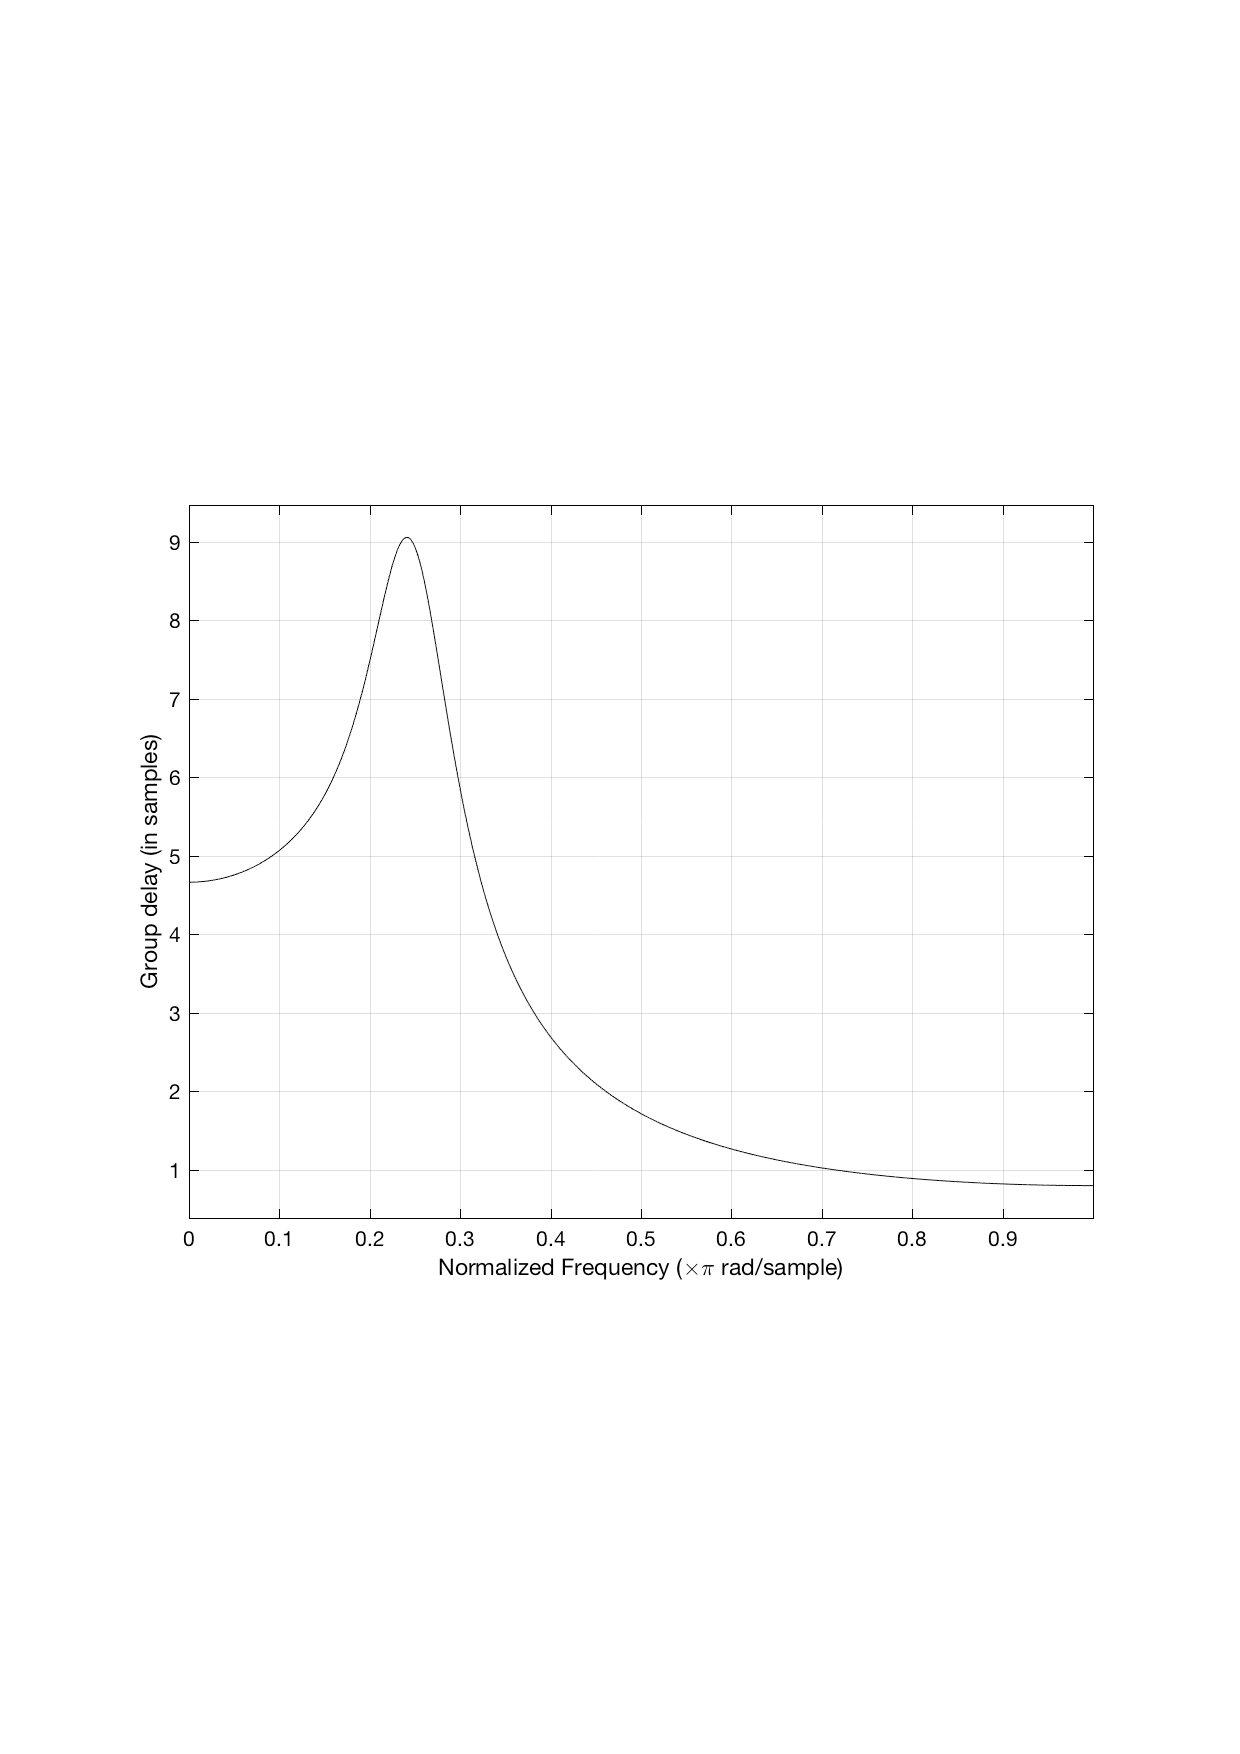
\includegraphics[width=\linewidth]{groupDelayIirPrev}
	\caption{Group delay of a 4th order IIR filter.}
	\label{fig:groupDelayIirPrev}
\end{subfigure}
\hspace{6mm} 
\begin{subfigure}[t]{0.47\textwidth}
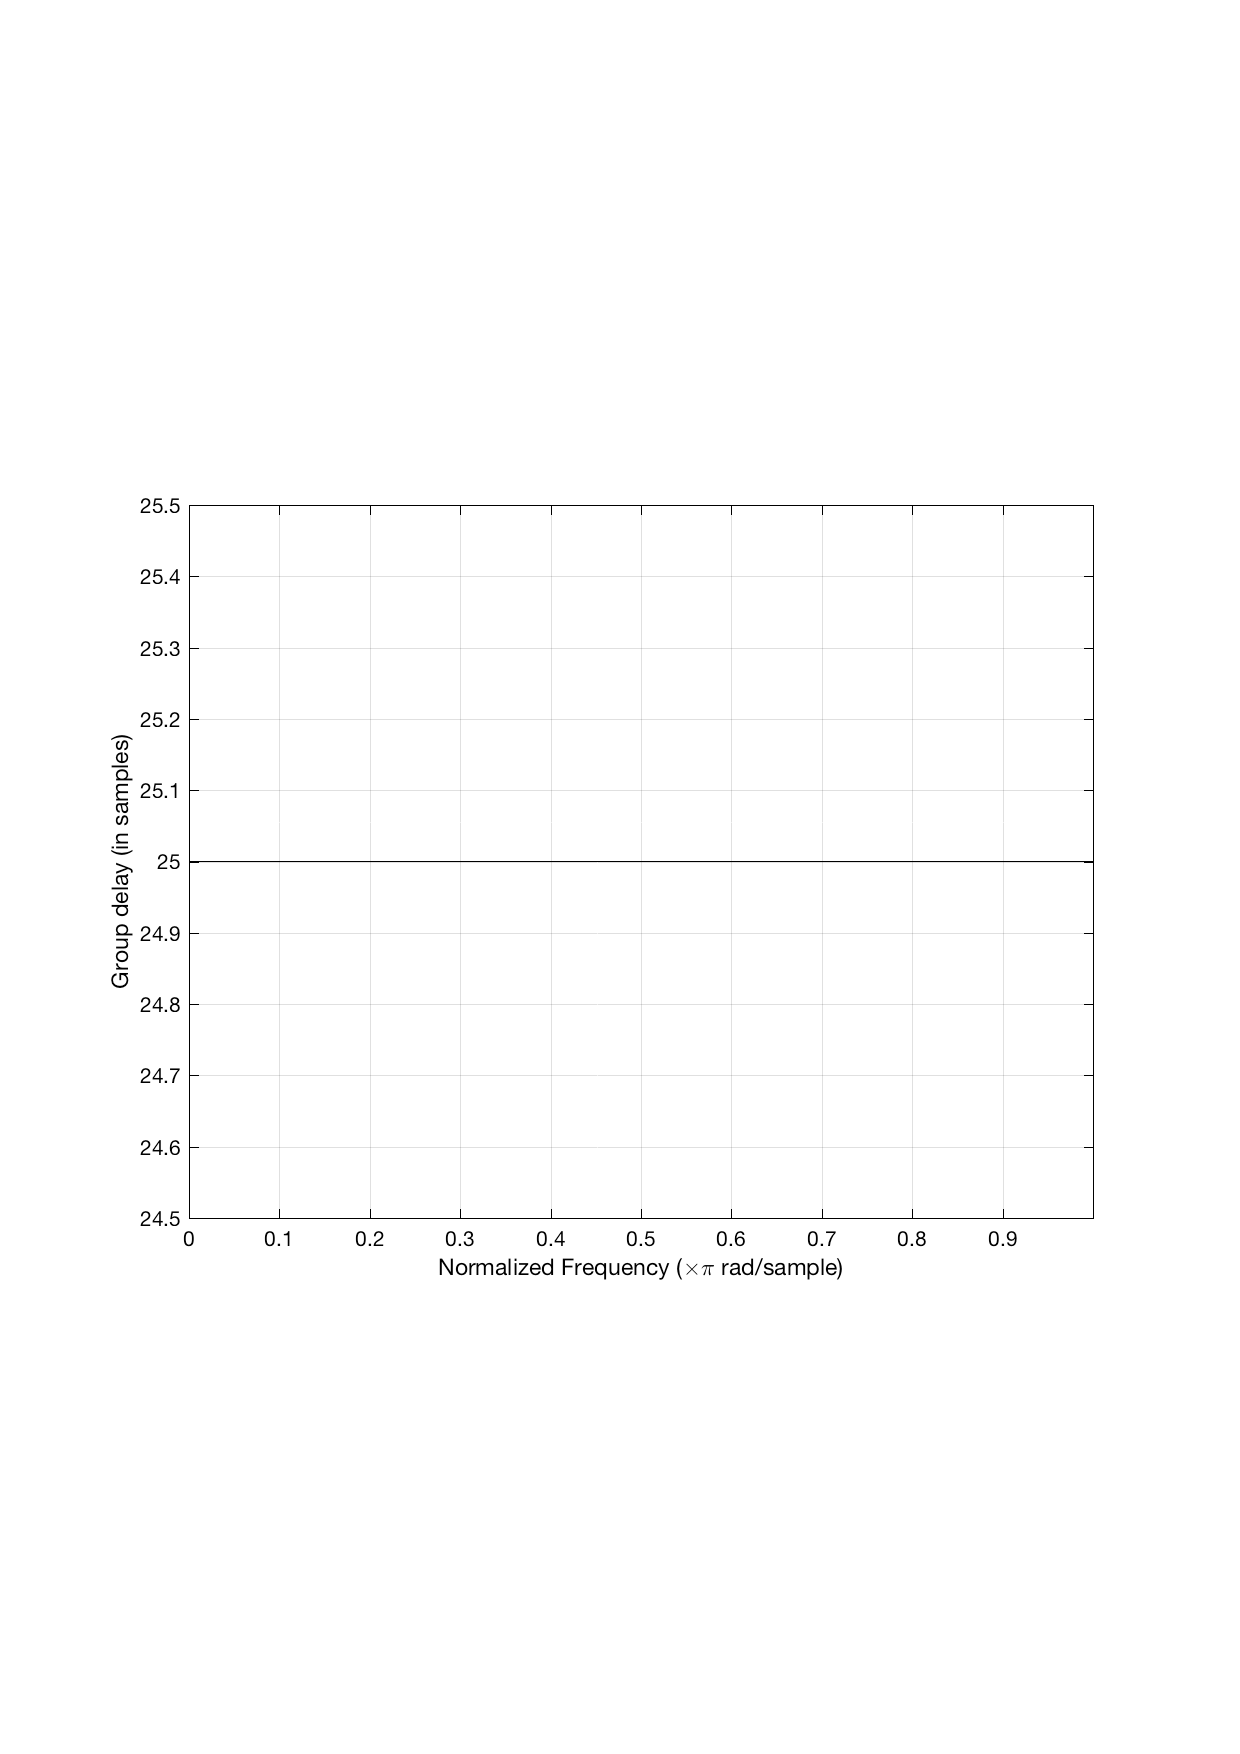
\includegraphics[width=\linewidth]{groupDelayFirPrev}
	\caption{Group delay of a 50th order FIR filter.}
	\label{fig:groupDelayFirPrev}
\end{subfigure}
\caption{Example of group delay of an IIR and a FIR filter.}
\label{fig:filterGroupDelay}
\end{figure}

The group delay is an important parameter to take into account, as it specifies the sample delay for each frequency. 1 sample delay is equivalent to 20.83 $\mu$s in a 48 kHz system. \autoref{fig:groupDelayIirPrev} shows that the group delay for IIR filters is non-linear with a peak at the normalized frequency 0.25 $\pi rad$. To calculate the time delay at 0.25 $\pi$ rad following expression can be used:
\begin{equation}
t_{d}= \frac{n_{s}}{f_s} \enhed{s}
\end{equation}
\begin{where}
\va{$n_{s}$}{is the number of samples delayed}{.}
\end{where}

A non-linear group delay will be hard to compensate compared to a constant group delay, thus a constant group delay is desirable. To achieve a constant group delay a linear phase filter is needed as the phase response is linear. Linear phase can be found in FIR filters and Bessel filters. Because of the constant group delay in linear phase filters, it eases the design as constant delays can be implemented to compensate for the phase shift in filters. Bessel filters have a constant group delay until the cutoff frequency and gets non-linear afterwards. Because the Bessel filter do not have a very sharp cutoff compared to other filter types, a high order Bessel filter will be needed. A high order IIR however has risk of being unstable. FIR filters are therefore chosen as they have all the required properties and do not get unstable. 


\section{Computational Constraints}
Another subject to consider is the constraints regarding computational power to perform filter algorithms. For FIR filters the amount of instructions to compute the filter output increases by the filter order, as calculating each tap in the filter is equal to a multiply and accumulate. Therefore even though a very high order filter in theory is realizable, the computational constraint needs to be considered. 

The performance of the DSP is 100 MIPS. At a sample rate of 48 kHz, this will result in approximately 2083 instructions available in-between each sample. A 10000 order FIR filter for instance is thus not realizable on the platform with a sampling rate of 48 kHz as the DSP will not finish calculating the filter output in time before the next sample. This is true because the fastest way to compute the convolution between the input signal x[n] and the impulse response h[n] is by using a Multiply-Accumulate (MAC) instruction which takes 1 clock cycle to perform if a single MAC is used. This gives a total number of 10000 clock cycles to perform one single convolution. Designing FIR filters will therefore be difficult as the cutoff frequencies for all required filters are very low relative to the sampling rate. A cutoff frequency located far from the sampling rate results in a long impulse response for a FIR filter. To a achieve a steep cut more samples of the impulse response are needed thus increasing the order of the filter. 

\section{Multirate Signal Processing with Multistages}
A solution to avoid very high order filters is to downsample the signal into a signal with a lower sampling rate. By downsampling the signal the impulse response of an equivalent FIR filter at the same cutoff frequency is shortened and the amount of taps is therefore reduced. In \autoref{fig:downsample_FIR} it is shown how decreasing the sampling rate by an integer factor of L is equivalent to increasing the cutoff frequency by a factor of L.

% vis fordele ved multirate
% - båndpas filter har en højere cutoff
% - Ulempe er anti aliserings filter --> Høj orden

\begin{figure}[H]
\centering
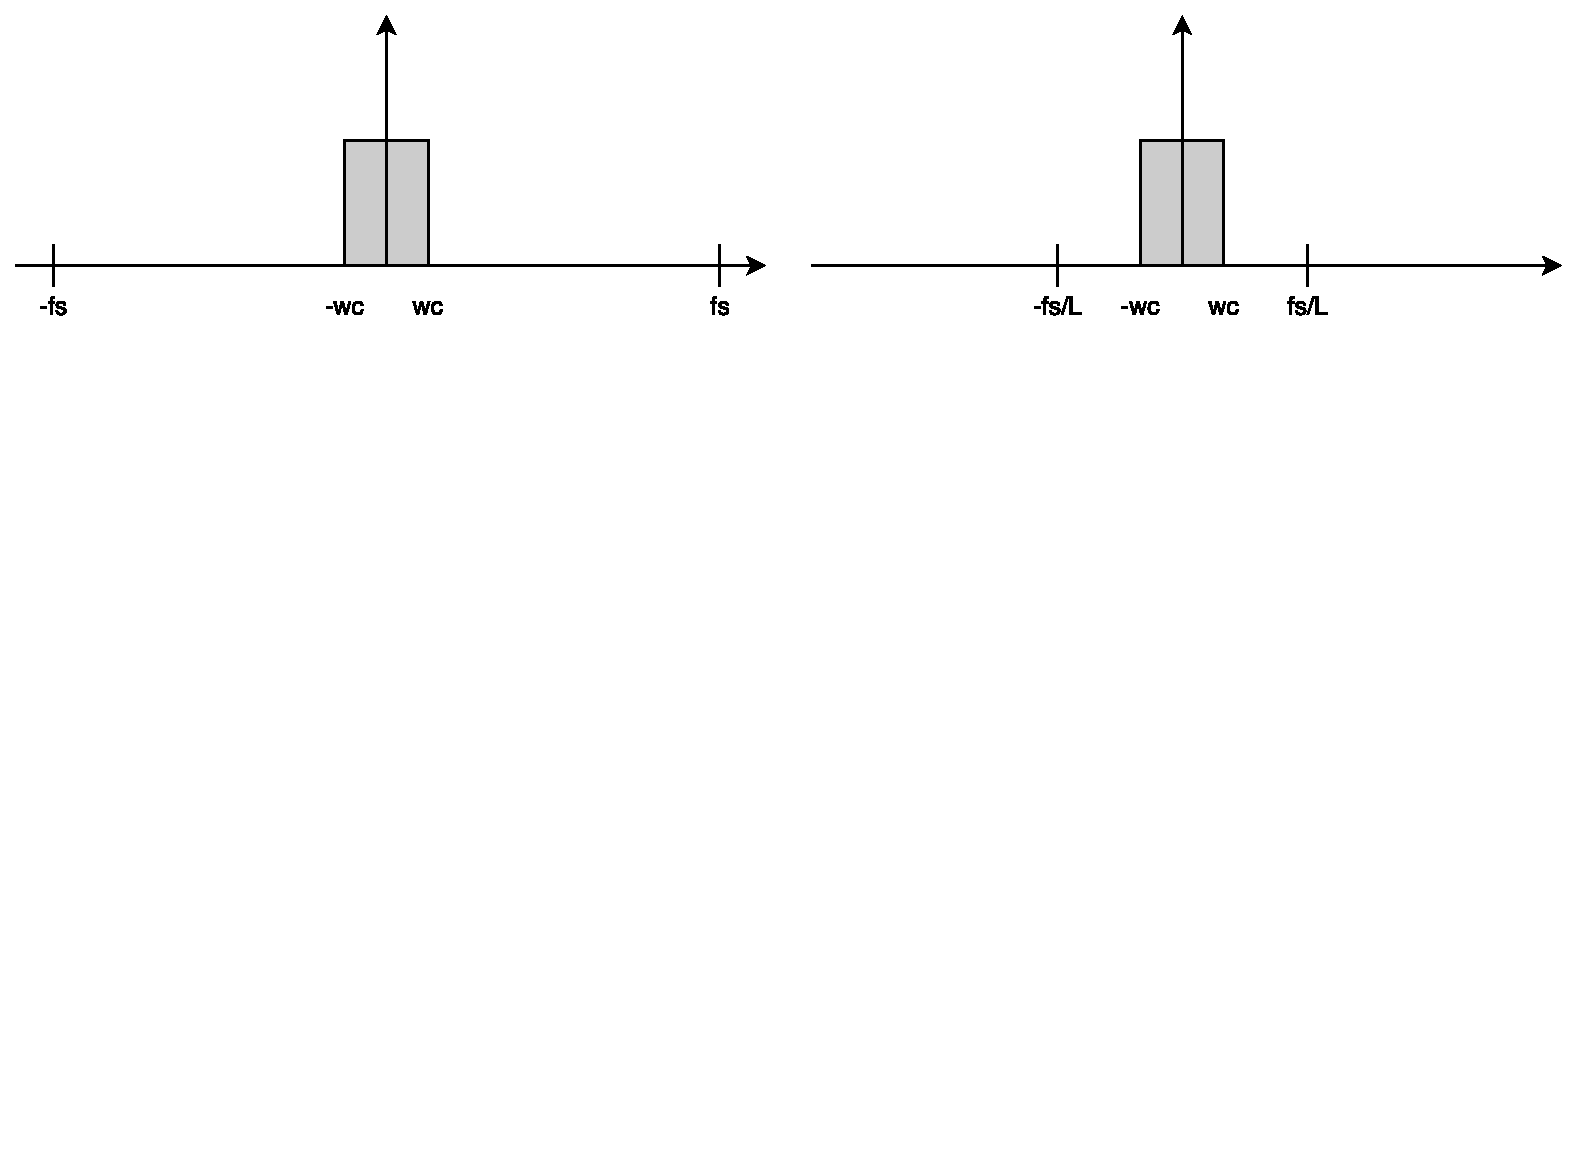
\includegraphics[width=0.75\textwidth]{figures/downsample_FIR.pdf}
\caption{Frequency spectrum of a signal with different sampling frequencies.}
\label{fig:downsample_FIR}
\end{figure}

An example of how to reduce the order of the FIR filter by multirate is shown in \autoref{fig:fir_downsample}. \autoref{fig:fir_downsample1} is a 100 order FIR filter with a sampling frequency of 48 kHz and cutoff frequency at $\frac{f_s}{10}$ and \autoref{fig:fir_downsample2} is a 50 order FIR filter with a sampling frequency of 24 kHz and cutoff frequency at $\frac{f_s}{5}$. 

\begin{figure}[H]
\centering
\begin{subfigure}[t]{0.44\textwidth}
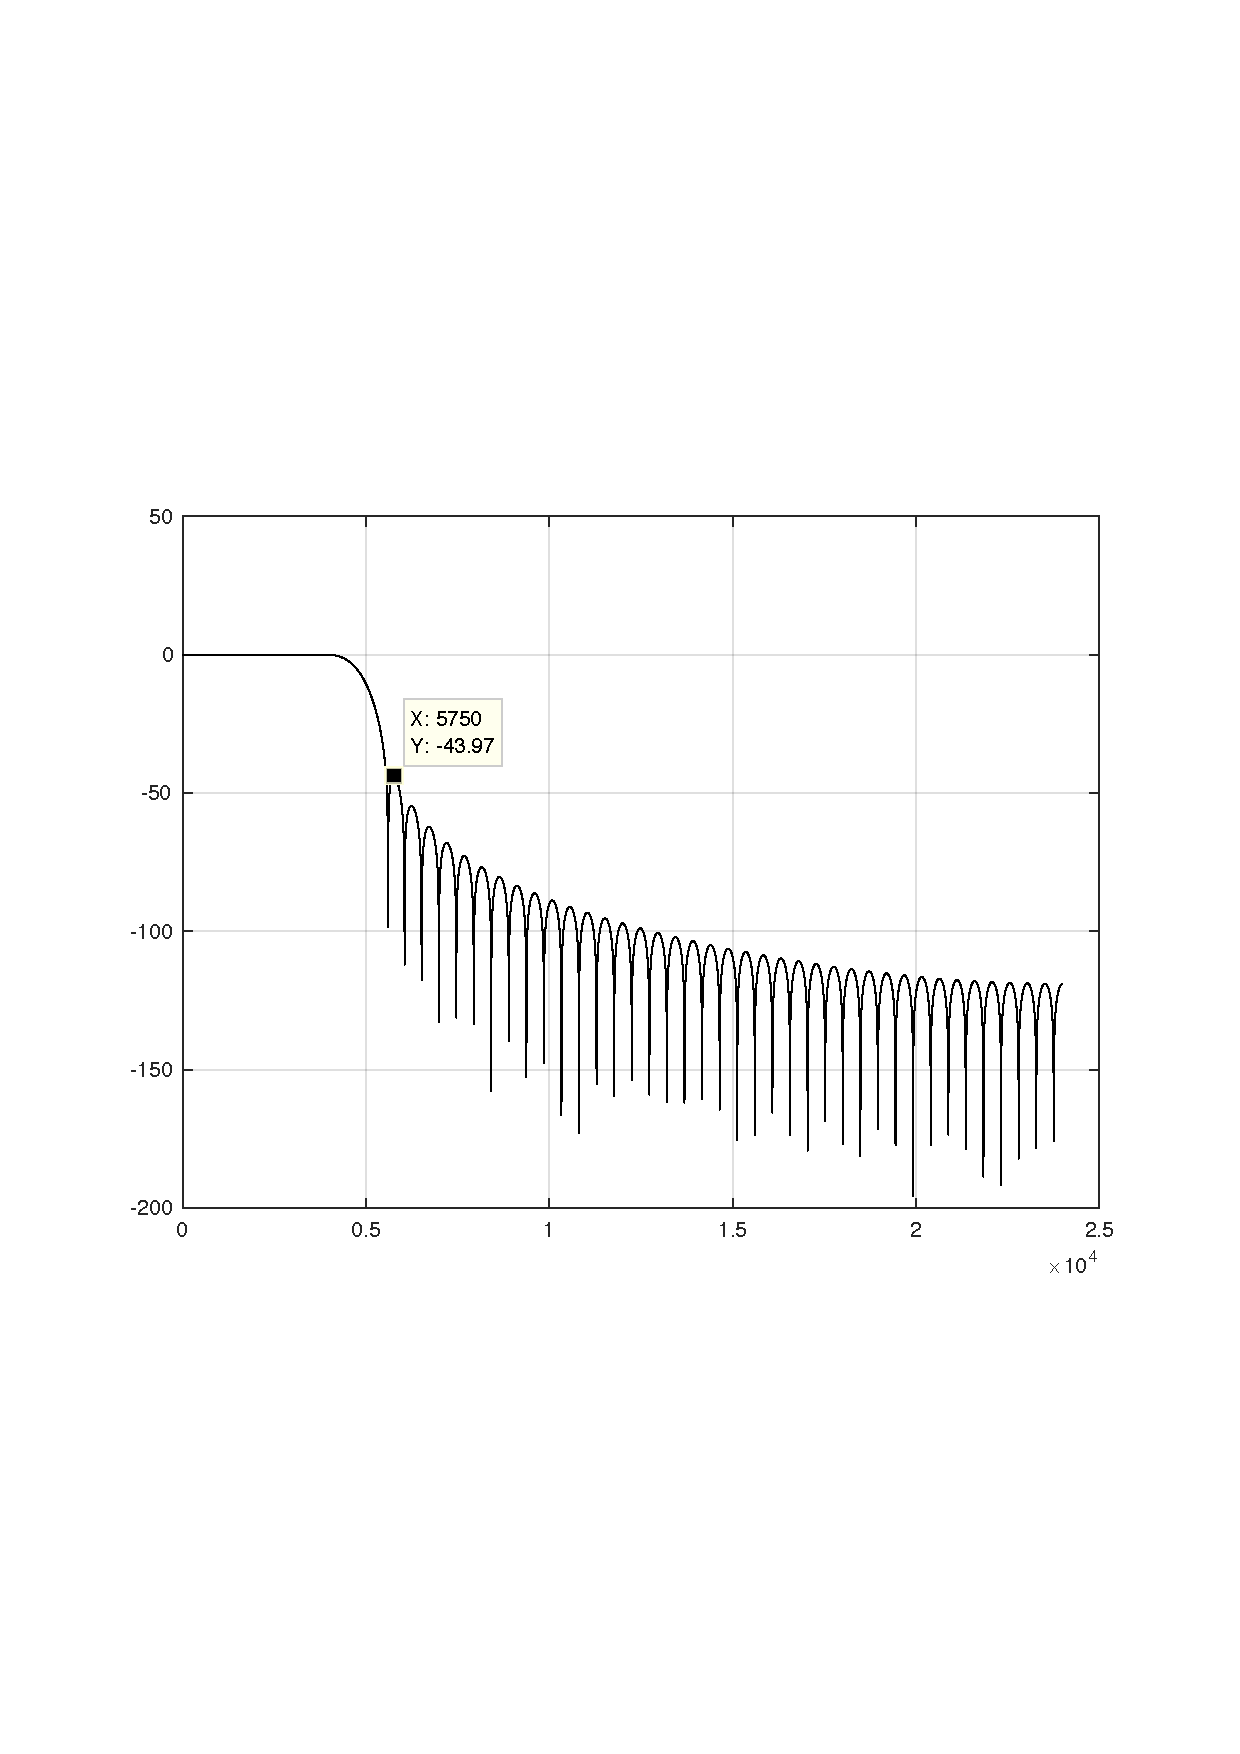
\includegraphics[width=\linewidth]{fir_downsample1}
	\caption{Frequency response of a FIR filter at $f_s$.}
	\label{fig:fir_downsample1}
\end{subfigure}
\hspace{6mm} 
\begin{subfigure}[t]{0.47\textwidth}
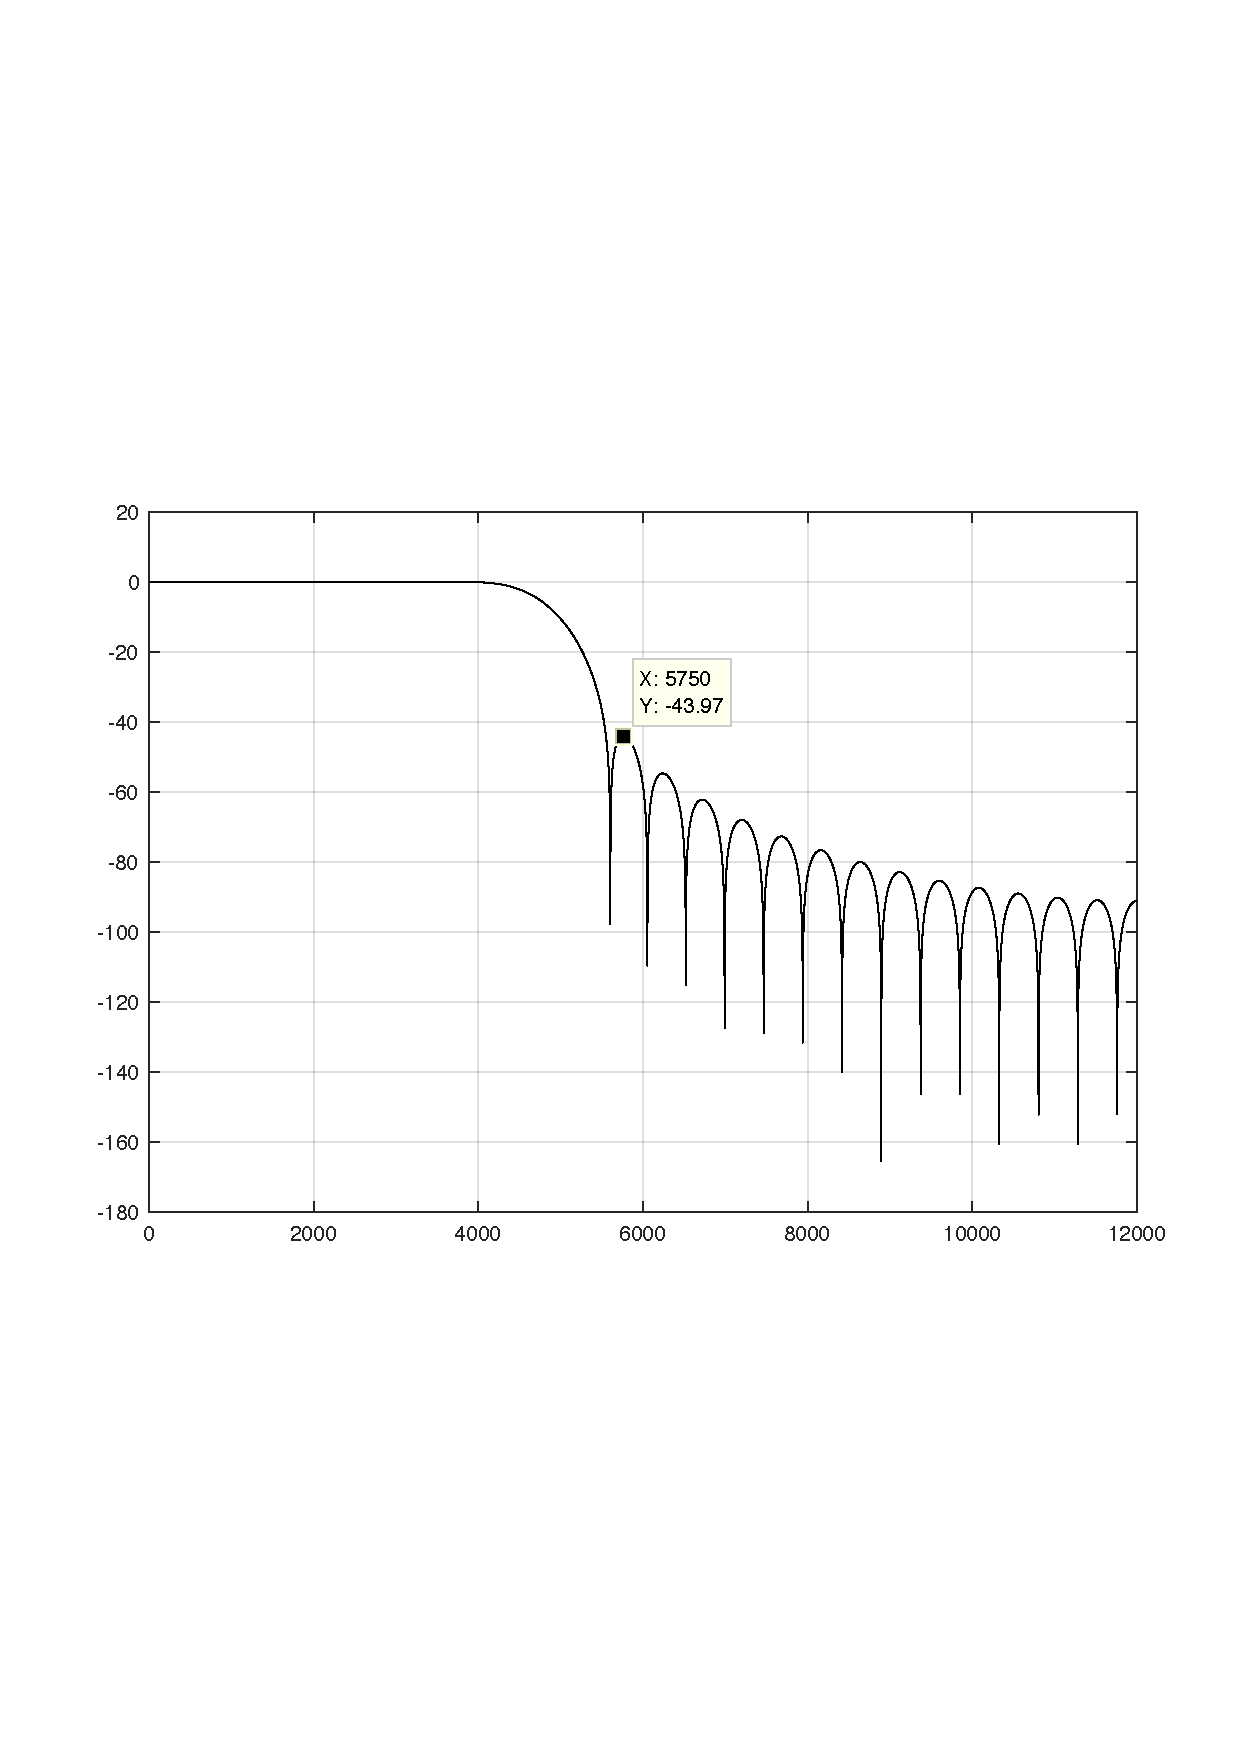
\includegraphics[width=\linewidth]{fir_downsample2}
	\caption{Frequency response of a FIR filter at $\frac{f_s}{2}$ with half the order.}
	\label{fig:fir_downsample2}
\end{subfigure}
\caption{Frequency response of two different FIR filters at different sampling frequencies.}
\label{fig:fir_downsample}
\end{figure}

It is seen that the attenuation at the top of the first side lope is -43.97 dB for both filters, thus the frequency response of both are the same at $0 \leq f \leq 24 \text{kHz}$. Because the frequency bands for the multi-band limiter are placed low, a multirate system will be implemented into the system as this helps decreasing the filter orders significantly.

%\subsection*{Avoiding Aliasing when Downsampling}
To downsample however requires an anti-aliasing filter to avoid aliasing as seen in \autoref{fig:aliasing}. The bandwidth of the audio signal is assumed to be 0 Hz to 20 kHz at a sampling rate of 48 kHz. The anti-aliasing filter has two requirements. The cutoff frequency should be low enough to limit the bandwidth and the attenuation at the new sampling rate $\frac{f_s}{2}$ should be high enough for aliasing not to occur. 

\begin{figure}[H]
\centering
\begin{subfigure}[t]{0.44\textwidth}
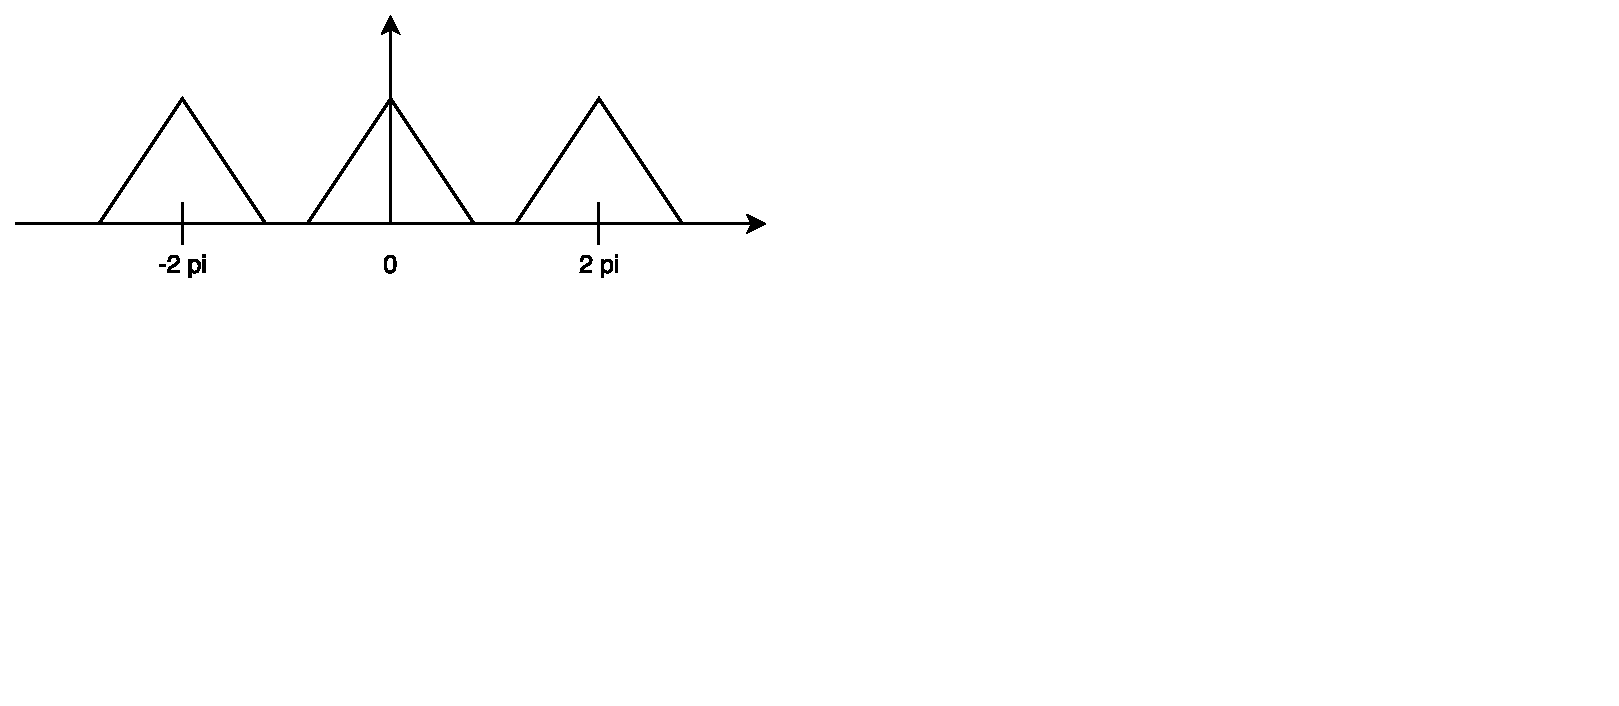
\includegraphics[width=\linewidth]{aliasing1}
	\caption{Signal bandwidth with sampling rate $f_s$.}
	\label{fig:aliasing1}
\end{subfigure}
\hspace{6mm} 
\begin{subfigure}[t]{0.47\textwidth}
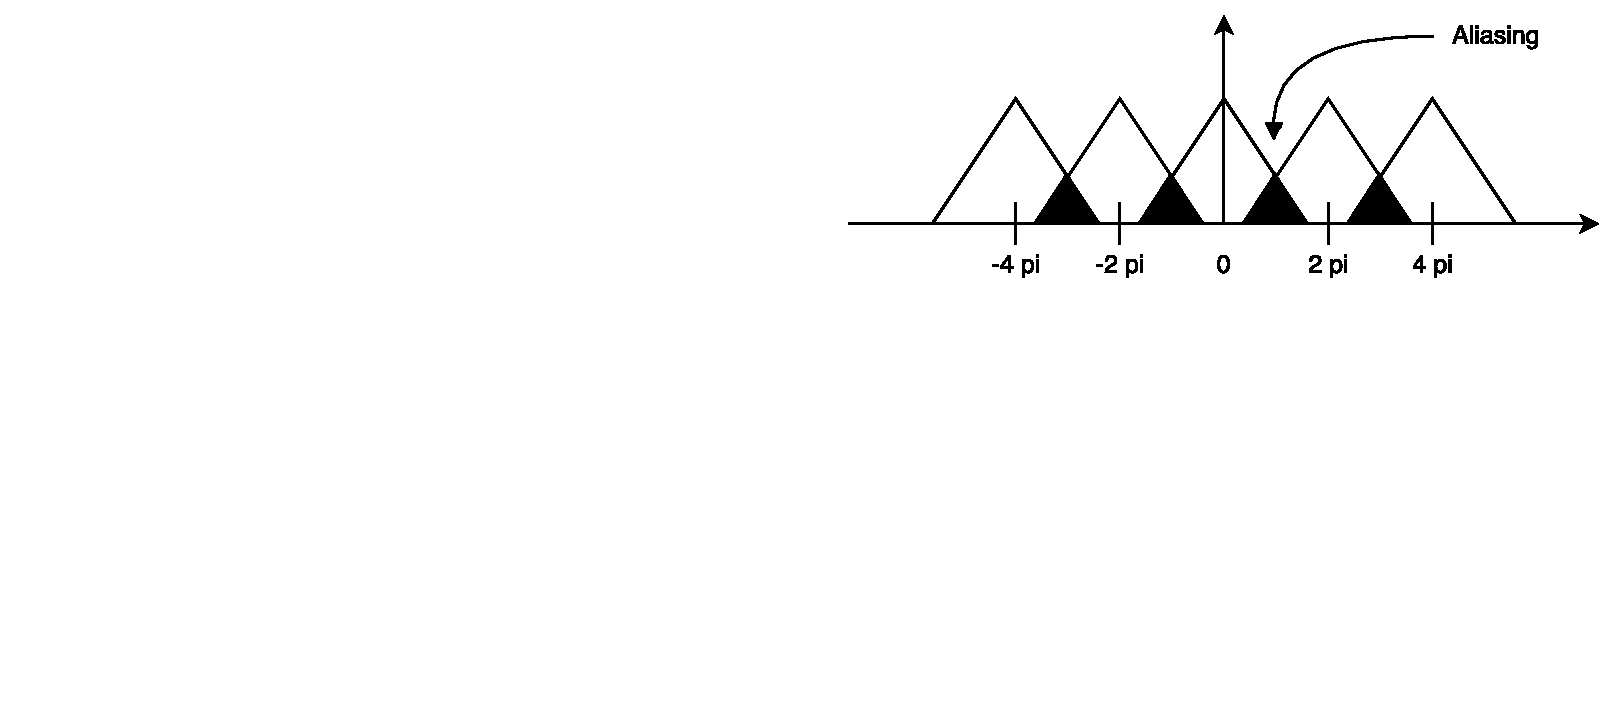
\includegraphics[width=\linewidth]{aliasing2}
	\caption{Aliasing occurs when downsampling to sampling rate $\frac{f_s}{L}$ without anti-aliasing filter.}
	\label{fig:aliasing2}
\end{subfigure}
\hspace{6mm}
\begin{subfigure}[b]{0.44\textwidth}
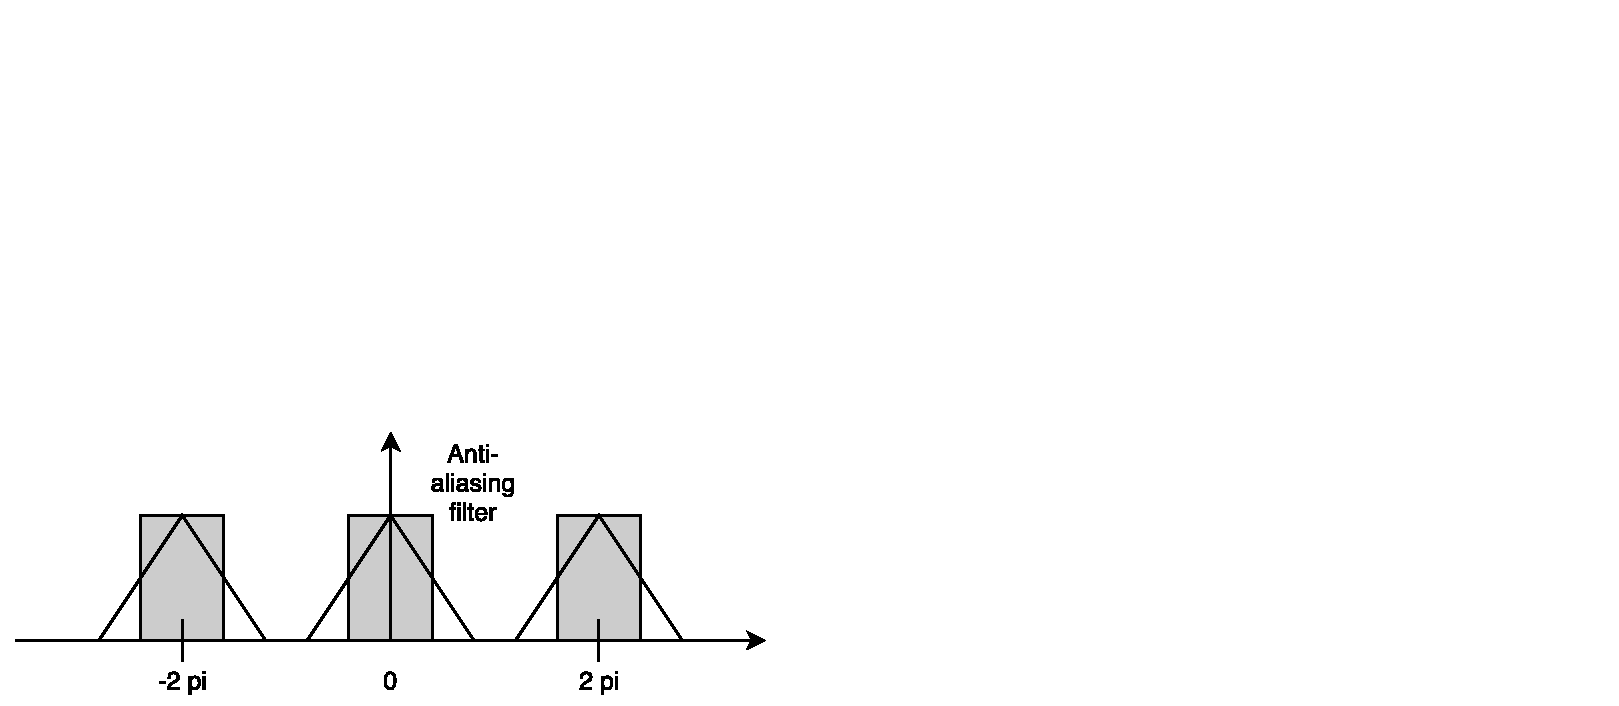
\includegraphics[width=\linewidth]{aliasing3}
	\caption{Aliasing filter applied to reduce the signal bandwidth.}
	\label{fig:aliasing3}
\end{subfigure}
\hspace{6mm} 
\begin{subfigure}[b]{0.47\textwidth}
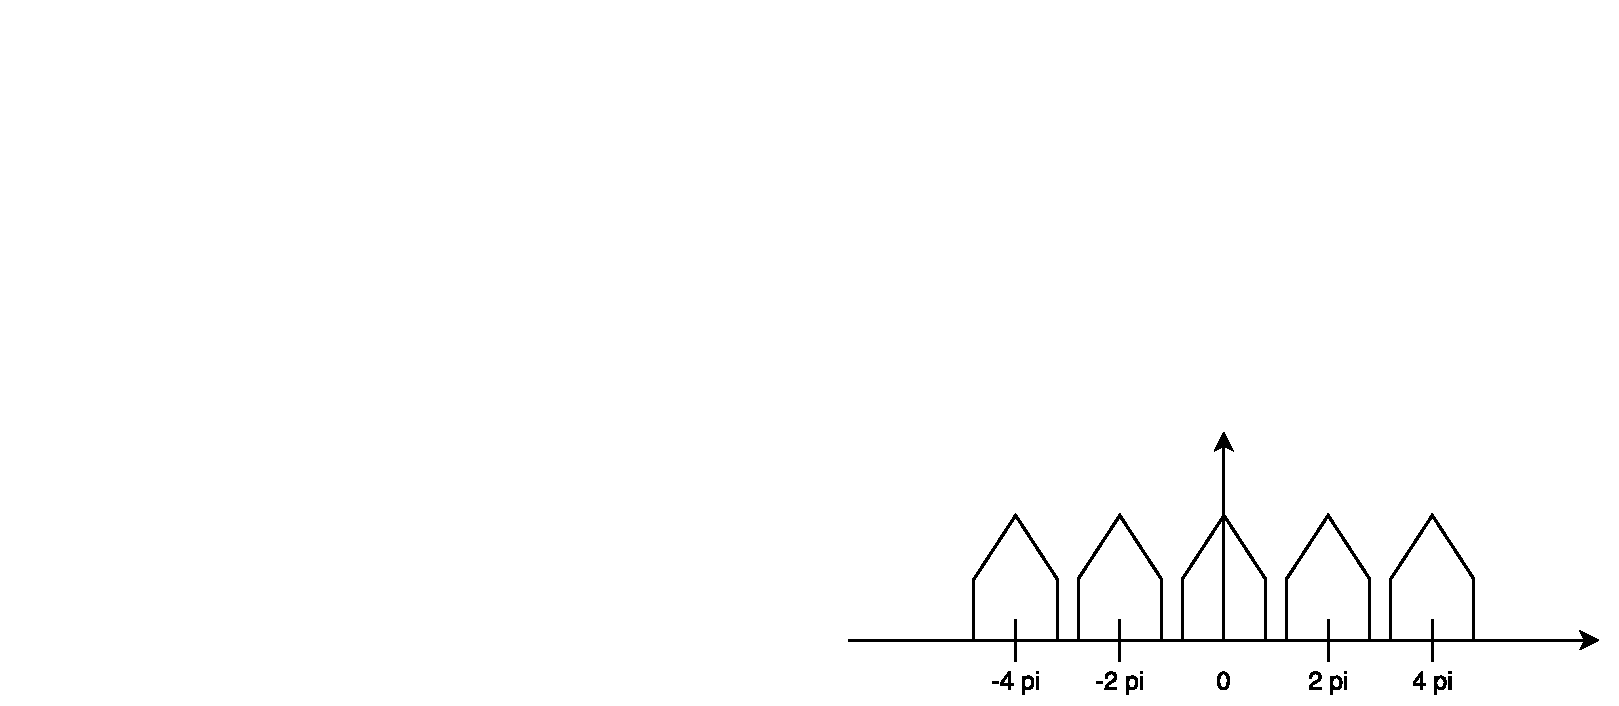
\includegraphics[width=\linewidth]{aliasing4}
	\caption{Aliasing at downsampling no longer occurs.}
	\label{fig:aliasing4}
\end{subfigure}
\caption{An anti-aliasing filter needs to applied to reduce the bandwidth to avoid aliasing when downsampling.}
\label{fig:aliasing}
\end{figure}

% Same number of taps required
If a high downsampling factor, L, is desired, then the order of the anti-aliasing filters will necessarily get bigger. A rule of thumb is the attenuation at $\frac{f_s}{2L}$ should approximately be -60 dB, since an ideal brick wall low-pass filter is not realizable. As the frequency bands for the system is located at the lower spectrum, a high order anti-aliasing filter is needed to downsample the signal. As a high order anti-aliasing filter is not desirable, the downsampling is performed in multistages to ease the amount of computation. If the downsampling is performed with a factor of 2 each time, then the total amount of computation needed to perform the filter algorithm for all stages pr. sample is given as a geometric series:

\begin{equation} \label{eq:z_transformation_example}
\sum_{k=0}^{\infty}M \left( \frac{1}{2} \right)^k  = \frac{M}{1-\frac{1}{2}} = 2M
\end{equation}
\begin{where}
\va{$M$}{is the filter order}{.}
\va{$k$}{is the number of downsamples}{.}
\end{where}

By doing so the filter order for each anti-aliasing filter is kept low as the cutoff frequency of each band is closer to the sampling frequency. Also, the whole bandwidth of the audio signal is split into octave bands which is an advantages if an equalizer and spectrum analyser are desired.

After downsampling, an upsampler is used to upsample the signal to the original sampling frequency. To upsample by a factor of L, L amount of zeros are inserted in-between each sample. This creates high frequency component that needs to be filtered to avoid artefacts from the mirrored spectrum. \autoref{fig:upsampling} illustrates the processes which is called interpolation

\begin{figure}[H]
\centering
\begin{subfigure}[t]{0.44\textwidth}
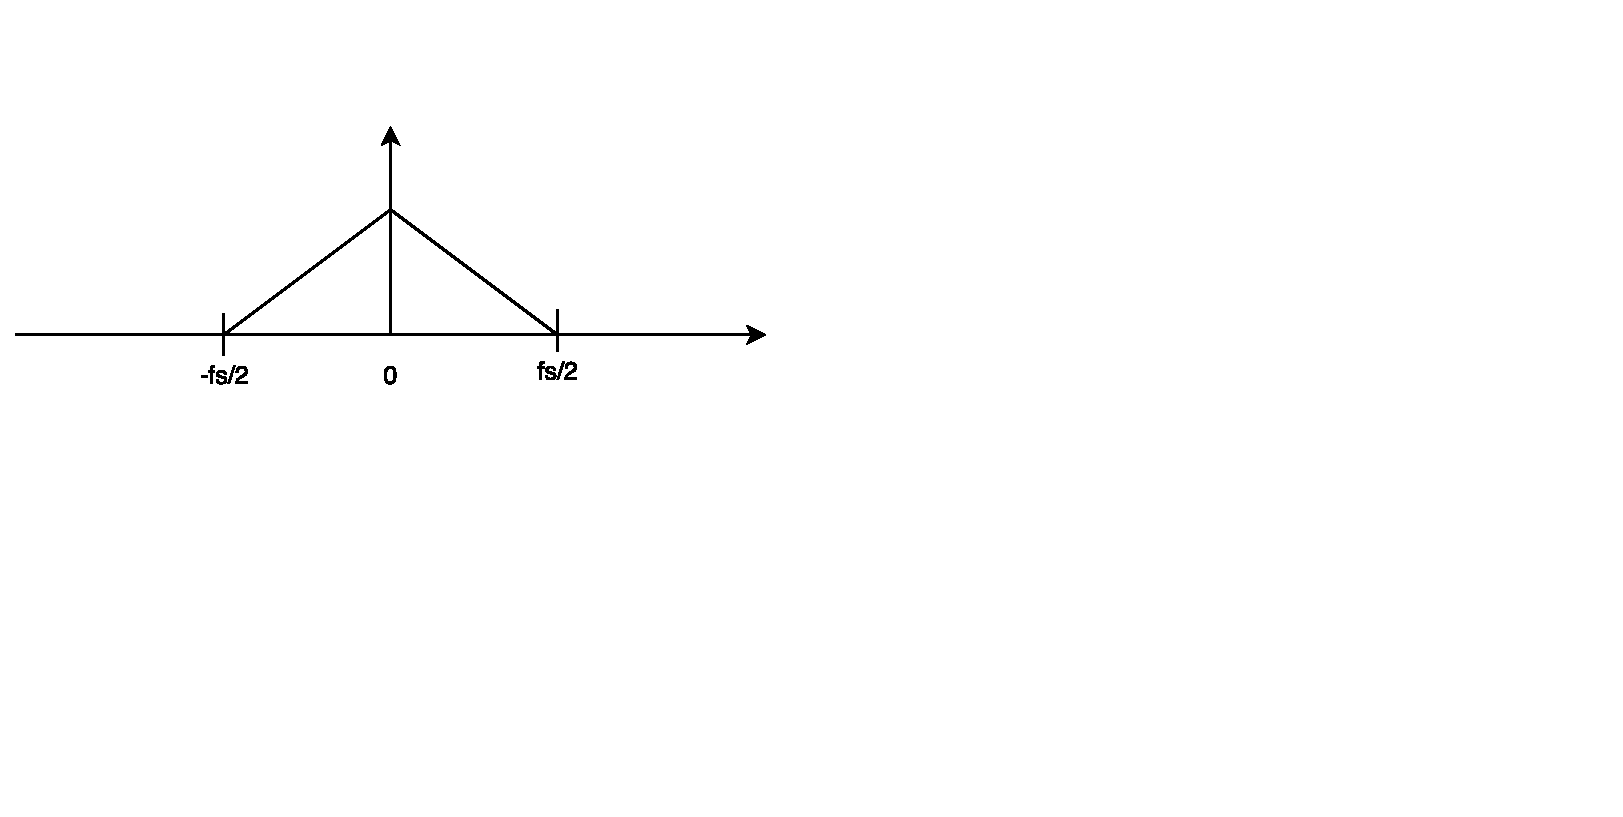
\includegraphics[width=\linewidth]{upsampling1}
	\caption{Signal bandwidth with sampling rate $f_s$.}
	\label{fig:upsampling1}
\end{subfigure}
\hspace{6mm} 
\begin{subfigure}[t]{0.47\textwidth}
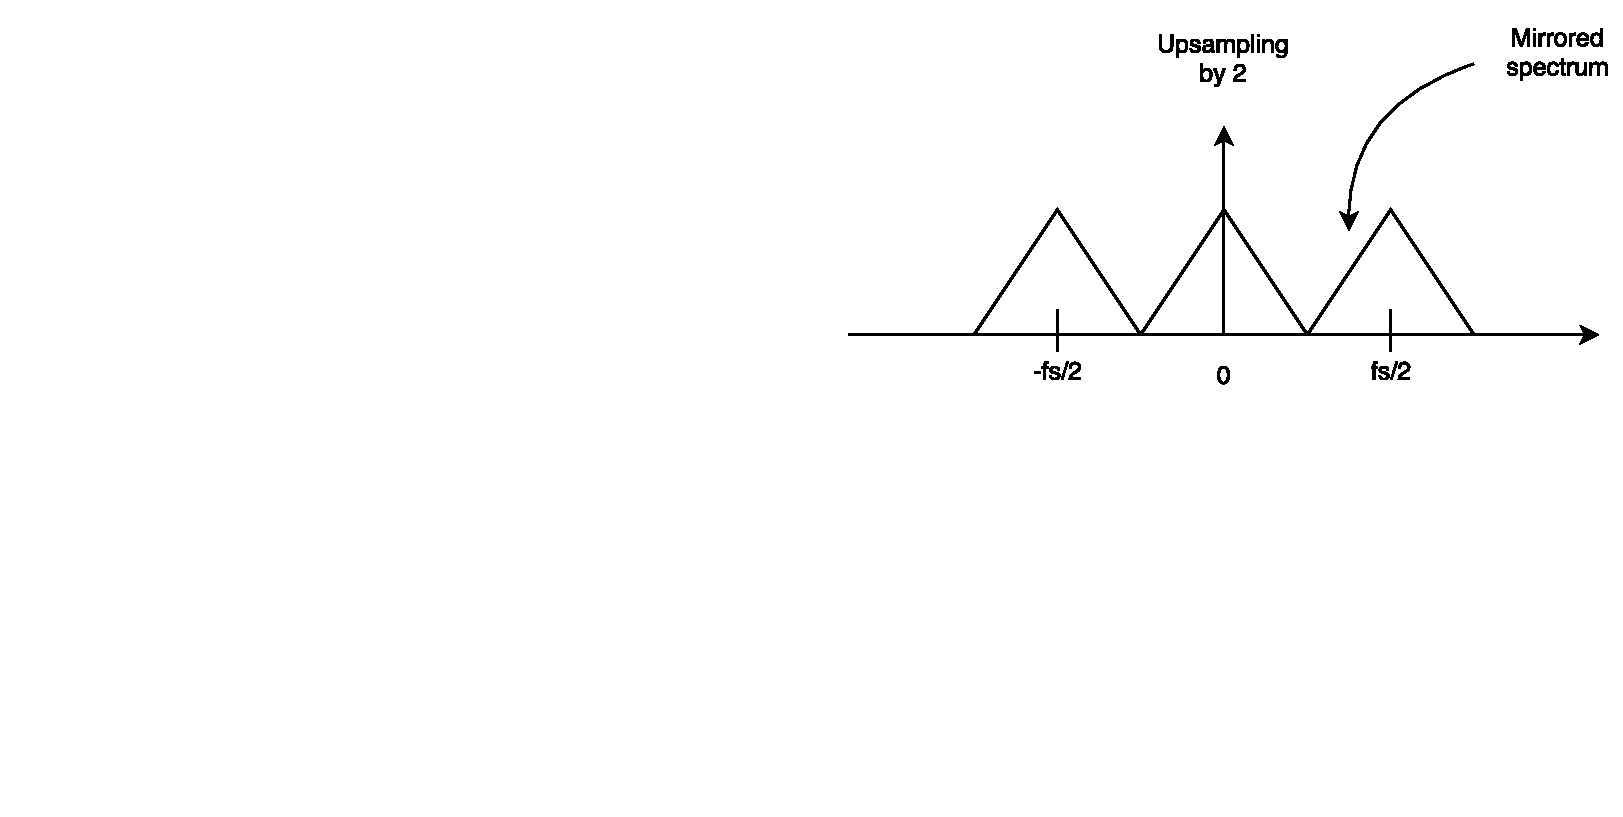
\includegraphics[width=\linewidth]{upsampling2}
	\caption{Upsampling mirrors the spectrum. The sampling frequency is increased by 2.}
	\label{fig:upsampling2}
\end{subfigure}
\hspace{6mm}
\begin{subfigure}[b]{0.44\textwidth}
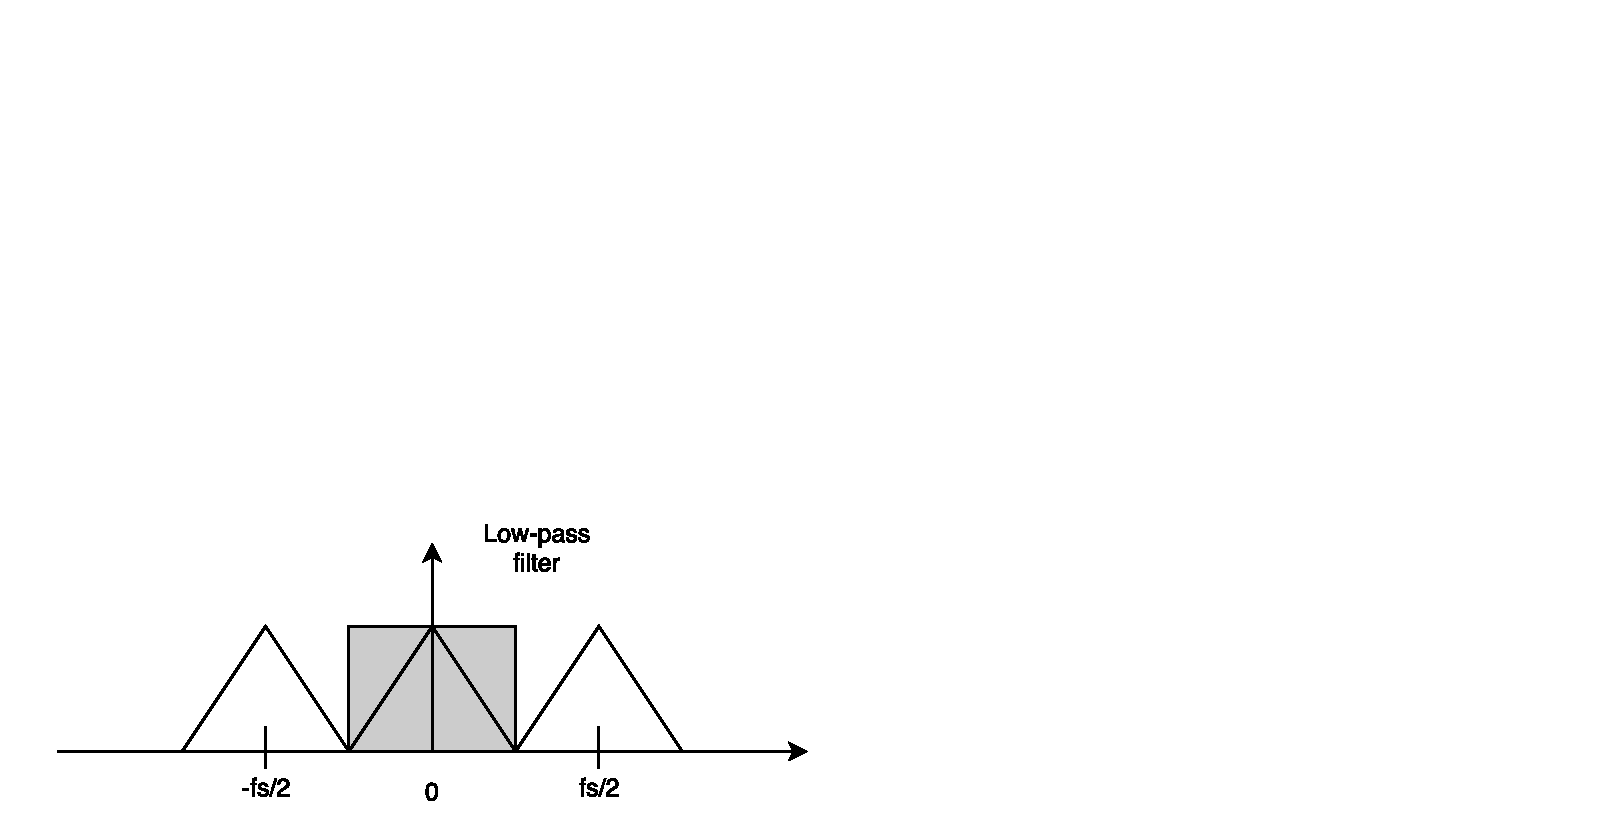
\includegraphics[width=\linewidth]{upsampling3}
	\caption{A low-pass filter removes artefacts from the mirrored spectrum.}
	\label{fig:upsampling3}
\end{subfigure}
\hspace{6mm} 
\begin{subfigure}[b]{0.47\textwidth}
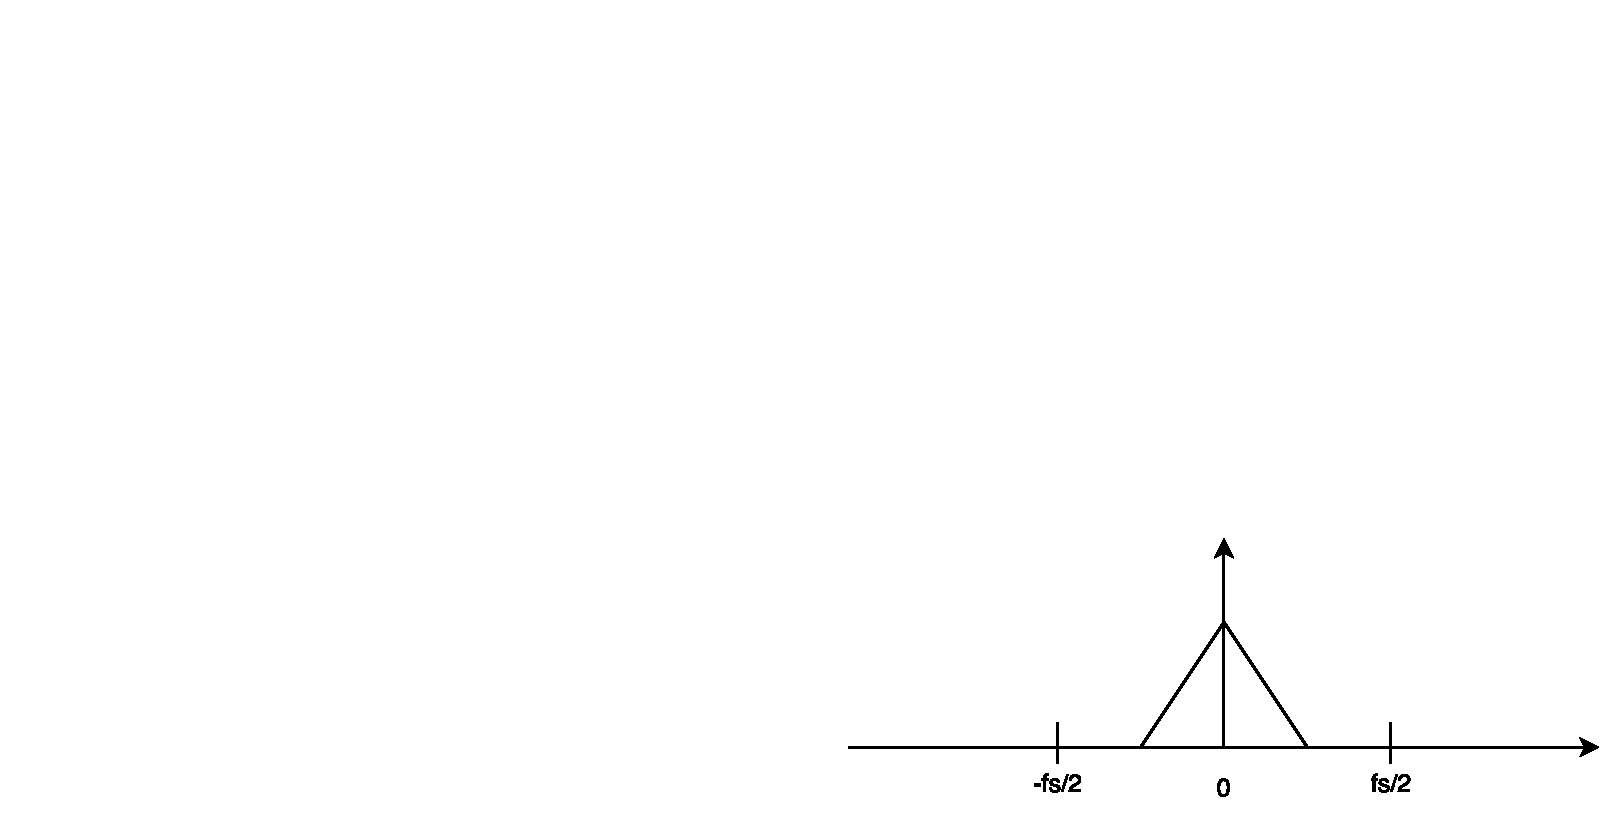
\includegraphics[width=\linewidth]{upsampling4}
	\caption{Aliasing at upsampling no longer occurs.}
	\label{fig:upsampling4}
\end{subfigure}
\caption{Processes of interpolation.}
\label{fig:upsampling}
\end{figure}






% Løsning:
% - Flere Downsamplings
% - Lavere ordens AA filtre
% - samlet samme orden, men AA-filtre ved lavere sampling frekvens skal processeres færre gange
% Processeringsmængden set fra den oprindelige samplingfrekvens er en geometrisk række

% Example downsample in 4 multistages vs 1 downsampling stage

Applying the considerations to the system, the following new overall system may be presented.

\begin{figure}[H]
\centering
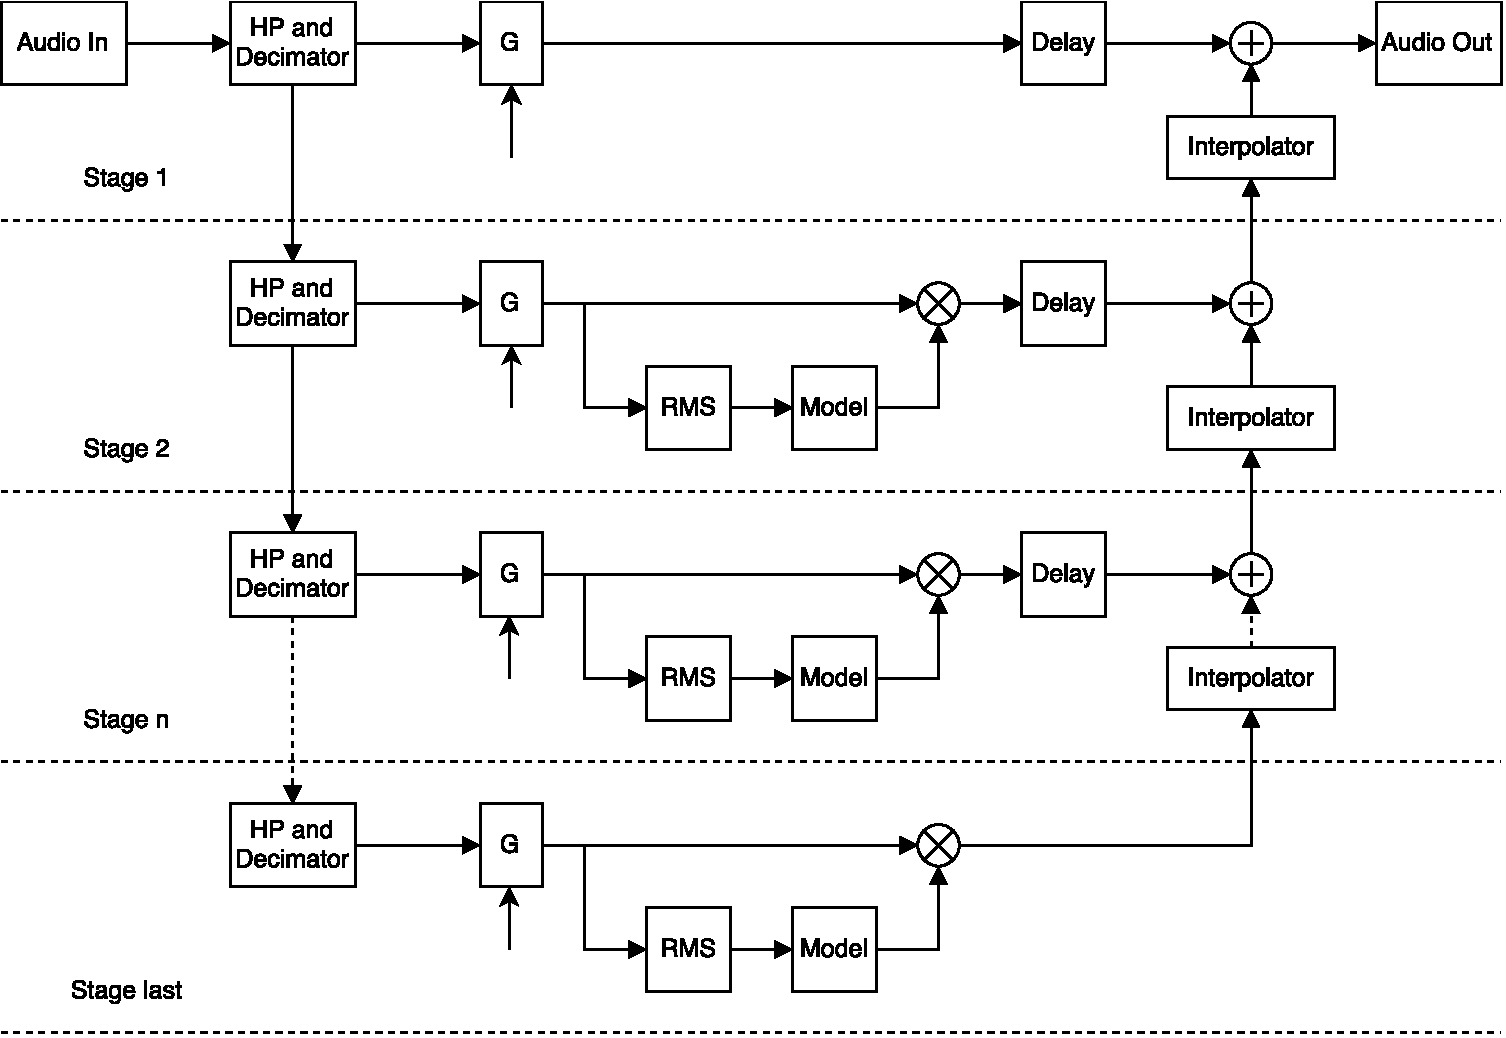
\includegraphics[width=0.75\textwidth]{figures/designRealBlock1.pdf}
\caption{Overall system with practical considerations.}
\label{fig:designRealBlock}
\end{figure}

In comparison to previous system overview, "HP and Decimator" and "interpolator" blocks are added to the system. The design of these blocks including the RMS and model will be discussed in following sections. 

Because a downsampling factor of 2 is used, the total amount of bands is 8, which means the equalizer to be designed has 8 adjustable bands.


\section{High-Pass Filter and Decimator}

A decimator is, as previously mentioned, a subsystem consisting of an anti-aliasing filter and a downsampler. As the anti-aliasing essentially is a low-pass filter, applying a design technique called spectral inversion, to the low-pass filtered signal results in high-pass filter. Applying this technique is equivalent to design a mirror filter of the low-pass filter. The technique saves the need for designing a mirror filter of the low-pass filter. The high-pass and decimation block is seen in figure \autoref{fig:designRealDecimator}.

\begin{figure}[H]
\centering
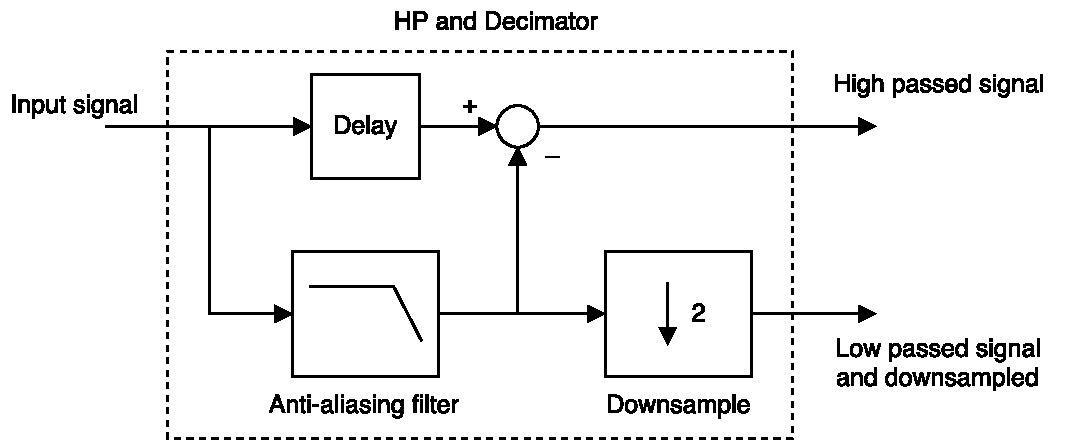
\includegraphics[width=0.75\textwidth]{figures/designRealDecimator.pdf}
\caption{The decimation block consist of a decimator and a spectral inversion to achieve a high-pass filter.}
\label{fig:designRealDecimator}
\end{figure}

A great advantage of using this technique rather than designing a mirror filter/highpass filter, is the algorithm to perform it, which is only a subtraction. To apply spectral inversion, a delay of the input signal before subtraction is required. This is due to the delay of the anti-aliasing filter.


\section{Interpolator}

Opposite to the decimator is the interpolator. As it is desired to reconstruct the signal, upsampling is applied to the downsampled signal. To upsample the downsampled signal, zero-padding is applied. Since the upsampling factor is 2, a zero is added in-between each sample. This adds high frequency components which is then filtered by using a low-pass filter. The requirement for the upsampling filter is that the attenuation at $\frac{f_s}{2}$ of the zero-padded signal is high enough to attenuate the mirrored spectrum and not influencing the bandwidth of the signal. The block diagram of the interpolator is seen in \autoref{fig:designRealInterpolator}.

\begin{figure}[H]
\centering
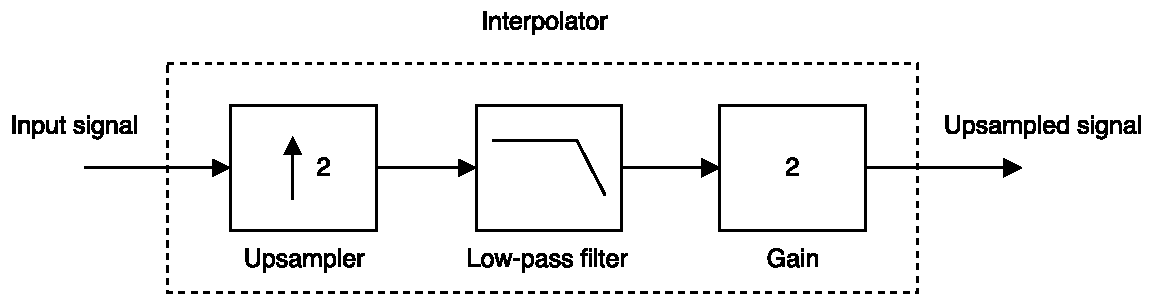
\includegraphics[width=0.75\textwidth]{figures/designRealInterpolator.pdf}
\caption{The interpolator consist of an upsampler, low-pass filter and a gain factor determined by the upsampling factor.}
\label{fig:designRealInterpolator}
\end{figure}

After low-pass filtering the signal, a gain of 2 corresponding to L is applied.


\section{RMS and Model}

To design an RMS limiter, an RMS analysis and a mathematical function of the gain is needed. For each band, the signal is fed into an RMS block, which calculates the RMS-value. The RMS-value is sent to a Model-block which checks if the RMS-value is above a defined threshold. If the RMS-value is above the threshold the model will apply a gain. If the RMS-value is below, the output will be a gain of 1. The block diagram of the RMS and model is seen in \autoref{fig:designRealRMS}.

\begin{figure}[H]
\centering
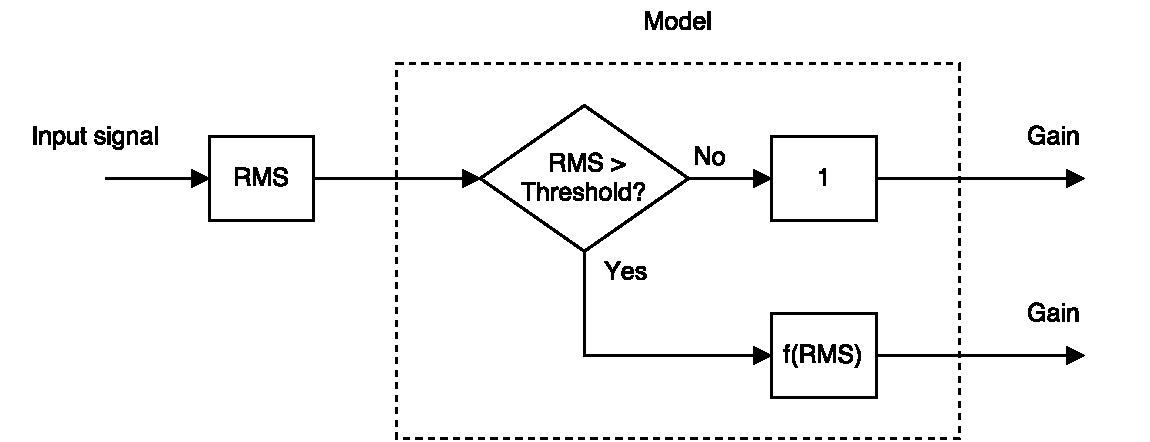
\includegraphics[width=0.75\textwidth]{figures/designRealRMS.pdf}
\caption{The RMS-value is first calculated and then fed into a subsystem that determines which gain to apply on the signal.}
\label{fig:designRealRMS}
\end{figure}

%To determine the threshold of the "model", a test of the loudspeaker needs to be done. The purpose of the test is to examine at which RMS-level the loudspeaker is either performing bad or damaging itself. To perform a RMS-analysis the minimum aount of samples needed is the amount of samples to represent the lowest frequency in that band. This introduces a small attact time, meaning the RMS-limiter cannot catch fast transients.



\section{Complete System}

The RMS limiter cannot protect the driver against transients such as kick drums and short spikes with high amplitude due to the attack time in the RMS calculation which is not instantanious. To avoid potential damage, a peak limiter is inserted in the upsampled 530 Hz band. The threshold of this limiter is set very high, as the main purpose it to protect the driver at cases where the RMS-limiter is not fast enough to respond. Another RMS-limiter is inserted in the upsampled 530 band. Because the signal is split into 4 bands, the 530 Hz band RMS-limiter ensures that the sum of all 4 bands do not exceed the threshold.

\begin{figure}[H]
\centering
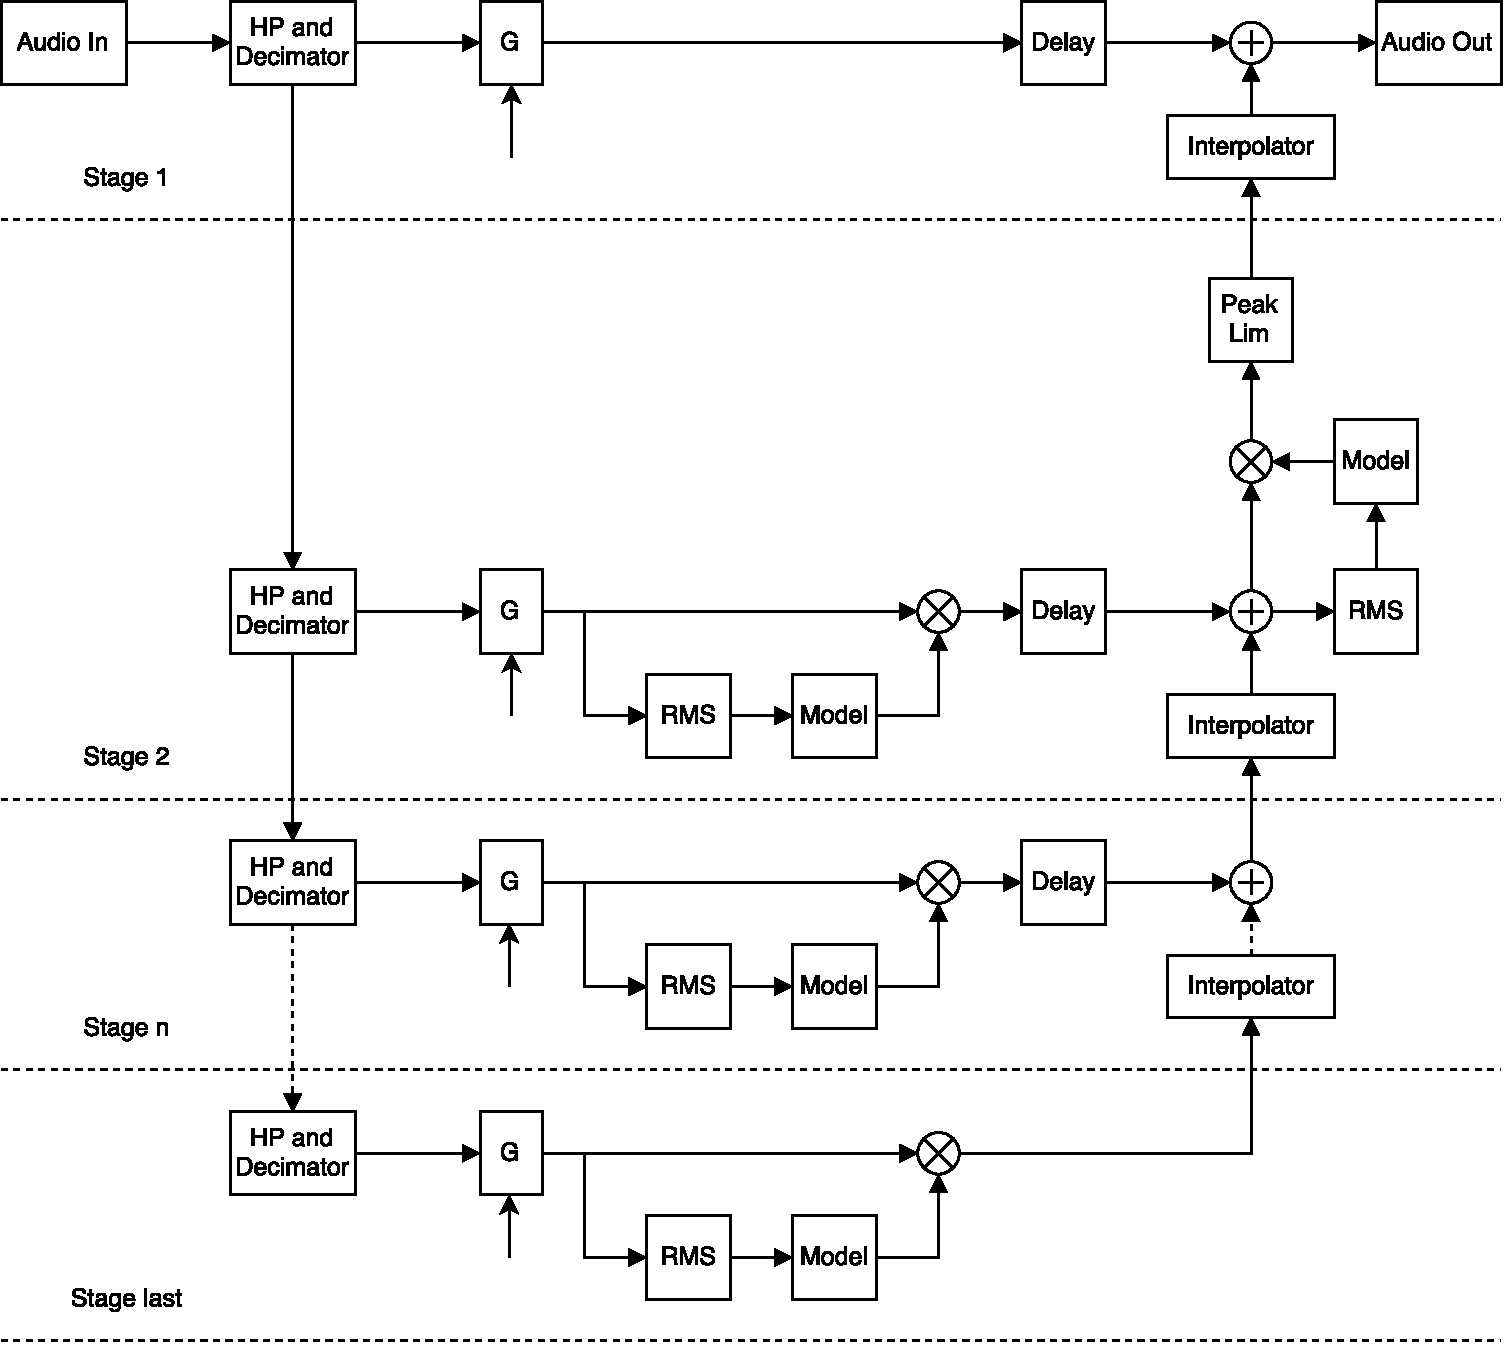
\includegraphics[width=0.75\textwidth]{figures/designRealFull.pdf}
\caption{The complete overall system to be designed.}
\label{fig:designRealBlock}
\end{figure}


The complete system is now explained and each subsystem of the system may now be designed in the following chapters.
